\section{Machine Learning and Predictive Modeling}
Machine learning enables computers to perform tasks without manually codifying all instructions.
This automated programming makes machine learning a popular and widely used approach for many applications as it provides a time- and cost-effective alternative to manually created software solutions.
Machine learning relies on algorithms that learn and generalize from examples in order to perform accurately on new or unseen data.

Predictive modeling is a subcategory of machine learning that aims to predict certain properties from given input data.
The input data typically consists of \emph{instances} with a given set of \emph{features}.
The values of those features can be binary, categorical, or numerical.
We can think of the data as a table where features are columns and rows are instances.
Thus, this kind of data is typically referred to as \emph{tabular} or \emph{structured} data.
In the case of \emph{unstructured} data, such as plain text, the data needs to be converted into structured data first, before it can be used as input of predictive models.
The predicted property, \emph{outcome} or \emph{label}, can be numerical, in which case the task is called \emph{regression}, or categorical, in which case the task is called \emph{classification}.
The different values the label can assume are called \emph{classes}.
The task is call \emph{binary classification} if the categorical label has exactly two classes.

The predictive model learns by \emph{training} with a set of example instances (\emph{training set}) and their associated labels.
In order to verify that the model did indeed correctly learn from the given examples, a second, previously unseen, set of example instances (training or \emph{validation set}) with known labels is typically used.
The model is used to predict the labels of this set which are then compared to the actual labels of those instances.
Various statistical measures can be computed on this relationship between the predicted and actual labels.

For binary classification tasks (for simplicity \emph{positive} and \emph{negative} are used below to describe the outcomes) those statistical measures include:

\begin{description}[noitemsep]
    \item[True Positive / Negative]
    The number of correctly predicted positive ($TP$) or negative instances ($TN$).
    \item[False Positive / Negative]
    The number of incorrectly predicted positive ($FP$) or negative instances ($FN$).
    \item[Accuracy]
    $(TP + TN) / (TP + TN + FP + FN)$ The proportion of correctly predicted instances.
    \item[Precision]
    $TP / (TP + FP)$ The ratio of correctly predicted positive instances to instances which were predicted to be positive.
    \item[True Positive Rate / Recall]
    $TP / (TP + FN)$ The proportion of correctly predicted positive instances.
    \item[False Positive Rate]
    $FP / (FP + TN)$ The proportion of incorrectly predicted positive instances.
\end{description}

Additionally, a further model quality measurement can be derived from the confidence of a model in its prediction.
Typically, classification models allow to output probabilities for each class instead of the predicted class directly.
This allows for inspecting the \emph{confidence} of the model.
In the case of binary classifiers a \emph{threshold} can be used to adjust predictions to favor confidence in a certain class higher than the other.
This is achieved by outputting the positive class as prediction if its probability is higher than the threshold and the negative class otherwise.

\begin{figure}
\centering
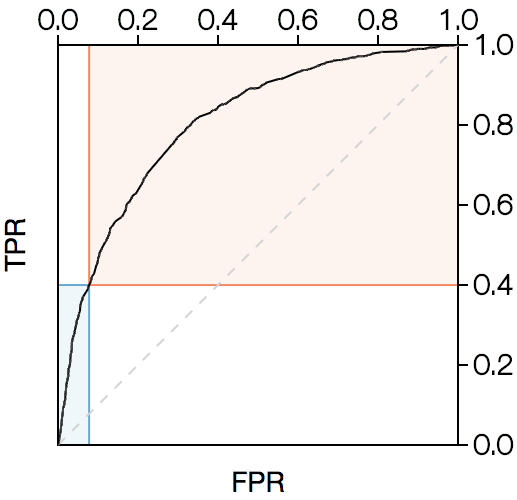
\includegraphics[height=10em]{figs/roc}
\caption[Example of a ROC curve.]{
Example of a ROC curve. The threshold minimizing incorrect predictions is highlighted by the colored axes.
}
\label{figs:roc_intro}
\end{figure}

The \emph{receiver operating characteristic} (ROC) curve for binary classifiers plots the true positive rate against the false positive rate for all thresholds between $0$ and $1$.
The plot indicates the correctness of the model \wrt its confidence.
The ROC curve for a perfect model ($100\%$ accuracy) would follow the left vertical axis and the top horizontal axis.
The area under the ROC curve (\emph{AUC}) is a commonly used measure for model quality. \todo{cite paper???}

\subsection{Popular Algorithms}
There are too many algorithms for predictive models to list all of them here.
However, following we will discuss the most commonly used algorithms.

\subsubsection{Logistic Regression}
\todo{log regr}
- logistic regression

\subsubsection{Additive Models}
\todo{additive models}

\subsubsection{Decision Trees}
\todo{decision trees}

\subsubsection{Ensemble Methods}
\todo{random forest / ensemble methods}

\subsubsection{Neural Networks}
\todo{neural network / multi-layer perceptron}

\subsection{Failure Modes}
\todo{failures}
- overfitting
- underfitting
- data
- model

\section{Visual Analytics}
% Visual analytics is the area of studying interactive graphical representations of abstract information with the help of computational and statistical procedures, in order to effectively analyze complex data. With regards to understanding the decision making of predictive machine learning models, there are two main strategies: white-box and black-box analysis \cite{class_signatures}.
\todo{visual analytics}
- use of high processing power of human eye
- interaction
- principles like Gestalt principles or preattentive perception or cleveland mcgill
% http://info.slis.indiana.edu/~katy/S637-S11/cleveland84.pdf
- ancombes quartett